%!TEX root = paper_ecg_cs_codec.tex
\section{Proposed Codec Architecture}
\label{sec:arch}

The ECG signal is split into windows
of $n$ samples each. The windows of
ECG signal are further grouped into
frames of $w$ windows each. The
last frame may have less than $w$
windows.
The encoder compresses the ECG signal
frame by frame.
The encoder converts the
ECG signal into a bitstream and the
decoder reconstructs the ECG signal
from the bitstream.

The encoder first sends
the encoder parameters in the form
of a stream header \cref{tbl:header:stream}.
Then for each frame of ECG signal,
it sends a frame header \cref{tbl:header:frame}
followed by a frame payload consisting of the
entropy coded measurements for the frame.

The encoding algorithm is presented in
\cref{alg:encoder}.
The decoding algorithm is presented in
\cref{alg:decoder}.

\subsection{Stream Header}
The stream header \cref{tbl:header:stream}
consists of all necessary information
required to initialize the decoder.
In particular, it contains the pseudo-random
generator key that can be used to reproduce
the sparse binary sensing matrix used in the
encoder by the decoder,
the number of samples per window ($n$),
the number of measurements per window ($m$),
the number of ones per column in the sensing matrix
($d$),
and the maximum number of windows in each frame
of ECG signal ($w$).
It contains a flag indicating whether adaptive
or fixed quantization will be used.
It contains the limits on the normalized
root mean square error for
the adaptive quantization ($\rho$)
and adaptive clipping ($\gamma$) steps.
If fixed quantization is used, then it contains
the fixed quantization parameter value ($q$).
Both $\rho$ and $\gamma$ in the stream header
are encoded using a simple decimal format $a 1e^{-b}$ where $a$
and $b$ are encoded as 4-bit integers.

Following \cite{mamaghanian2011compressed},
we construct a sparse binary sensing matrix $\Phi$ of shape
$m \times n$.
Each column of $\Phi$ consists of exactly $d$ ones and
$m-d$ zeros, where the position of ones has been randomly
selected in each column. Identical algorithm is used
to generate the sensing matrix using the stream header
parameters in both the encoder and the decoder.
The randomization is seeded with the parameter $\mathrm{key}$
sent in the stream header.

%!TEX root = ../paper_ecg_cs_codec.tex
\begin{table}[ht]
\centering
\caption{Stream header}
\begin{tabular}{llr}
\toprule
Parameter & Description & Bits \\
\midrule 
key & Pseudorandom generator key for $\Phi$ & 64 \\
$n$ & Window size & 12 \\
$m$ & Number of measurements per window & 12 \\
$d$ & Number of ones per column in sensing matrix & 6 \\
$w$ & Number of windows per frame & 8 \\
adaptive & Adaptive or fixed quantization flag & 1 \\
if (adaptive ) &  \\
\hspace{1cm} $\rho$ & $\nrmse$ limit for adaptive quantization & 8 \\
else & \\
\hspace{1cm} $q$ & Fixed quantization parameter & 4 \\
$\gamma$ & $\nrmse$ limit for clipping & 8 \\
\bottomrule
\end{tabular}
\label{tbl:header:stream}
\end{table}

%!TEX root = ../paper_ecg_cs_codec.tex
\begin{table}[ht]
\centering
\caption{Frame header}
\begin{tabular}{llr}
\toprule
Parameter & Description & Bits \\
\midrule

$\mu_y$ & Mean value & 16\\
$\sigma_y$ & Standard deviation & 16 \\
$q$ &  Frame quantization parameter & 3\\
$r$ &  Frame range parameter & 4 \\
$n_w$ & Windows in frame & 8 \\
$n_c$ & Words of entropy coded data& 16 \\
\bottomrule
\end{tabular}
\label{tbl:header:frame}
\end{table}


\subsection{Encoding}
\begin{figure}[!ht]
\centering 
%!TEX root = ../paper_ecg_cs_codec.tex
\begin{tikzpicture}[
scale=0.6, every node/.style={transform shape},
node distance=10mm and 10mm,
% basic style
cell/.style = {
    align=center,
    minimum width=2cm,
    minimum height=1cm
},
% normal blocks
block/.style= {cell, draw, shape=rectangle},
]
% Write your diagram code here
\node[cell](src){Digital\\Samples};
\node[block, right=of src](win){Windowing};
\node[block, right=of win](cs){Compressive\\Sensing};
\node[block, right=of cs](fl){Flattening};
\node[block, below=of win](q){Adaptive\\Quantization};
\node[block, right=of q](cl){Adaptive\\Clipping};
\node[block, right=of cl](ec){Entropy\\Coding};
\node[cell, right=of ec](cb){Compressed\\Bits};

% paths
\path[draw,->]
(src) edge (win)
(win) edge (cs)
(cs) edge (fl)
(q) edge (cl)
(cl) edge (ec)
(ec) edge (cb);

\draw[->] (fl.south) -- +(0, -3mm) -| (q.north);
\end{tikzpicture}


\caption{Digital Compressive Sensing Encoder}
\label{fig:cs:encoder}
\end{figure}


\begin{figure}[!t]
 \removelatexerror
 \centering
%!TEX root = ../paper_ecg_cs_codec.tex
\begin{algorithm}[H]
\caption{Encoder algorithm}
\label{alg:encoder}
\footnotesize
\SetAlgoLined
Send stream header \;
Build sensing matrix $\Phi$\;
\ForEach {frame of digital signal as $\bx$ with $n_w$ windows} {
    $\bX \leftarrow \window(\bx)$ \;
    \tcp{Sense}
    $\bY \leftarrow \Phi \bX$\;
    $\by \leftarrow \flatten(\bY)$\;
    \tcp{Adaptive quantization}
    \For{$q=q_{\max} \dots q_{\min}$ (descending)}{
        $\bar{\by} \leftarrow \left \lfloor \frac{1}{2^q}{\by} \right \rfloor$\;
        $\tilde{\by} \leftarrow 2^q \bar{\by}$\;
        \If{$\nrmse(\by, \tilde{\by}) \leq \rho$}{
            break \;
        }
    }
    \tcp{Quantized Gaussian model parameters}
    $\mu_y \leftarrow \left \lceil \text{mean}(\bar{\by}) \right \rceil$ \;
    $\sigma_y \leftarrow \left \lceil \text{std}(\bar{\by}) \right \rceil$ \;
    \tcp{Adaptive range adjustment}
    \For{$r=2 \dots 8$} {
        $y_{\min} \leftarrow \mu_y  - r \sigma_y$ \;
        $y_{\max} \leftarrow \mu_y  + r \sigma_y$ \;
        $\hat{\by} \leftarrow \clip(\bar{\by}, y_{\min}, y_{\max})$\;
        \If{$\nrmse(\bar{\by}, \hat{\by}) \leq \gamma$}{
            break \;
        }
    }
    $\bc \leftarrow \text{ans\_code}(\hat{\by}, \mu_y, \sigma_y, y_{\min}, y_{\max})$ \;
    $n_c \leftarrow$ number of words in $\bc$\;
    Send frame header($\mu_y, \sigma_y, q, r, n_w, n_c$)\;
    Send frame payload($\bc$)\;
}
\end{algorithm}

\end{figure}

Here we describe the encoding process for each frame.
\Cref{fig:cs:encoder} shows a block diagram of the frame encoding process.
The input to the encoder is a frame of digital ECG samples
at a given sampling rate $f_s$. In the MIT-BIH database,
the samples are digitally encoded in 11 bits per sample (unsigned).
Let the frame of ECG signal be denoted by $\bx$.
The frame is split into non-overlapping windows of $n$
samples each. We shall denote each window of $n$ samples
by vectors $\bx_i$. 

\subsubsection{Windowing}
A frame of ECG consists of multiple
such windows (up to a maximum of $w$ windows per
frame as per the encoder configuration).
Let the windows by denoted by $\bx_1, \bx_2, \dots$.
Let there be $w$ such windows.
We can put them together to form the (signed) signal matrix
\footnote{
PhysioNet provides the baseline values for each channel
in their ECG records.
Since the digital samples are unsigned, we have subtracted
them by the baseline value ($1024$ for 11-bit encoding).
11 bits mean that unsigned values range from
$0$ to $2047$. The baseline for zero amplitude is
digitally represented as $1024$.
After baseline adjustment, the range of values becomes
$[-1024,1023]$.
}:
\begin{equation}
\bX = \begin{bmatrix}
\bx_1 & \bx_2 & \dots & \bx_w
\end{bmatrix}.
\end{equation}

\subsubsection{Compressive Sensing}
The digital compressive sensing
is represented as
\begin{equation}
\by_i = \Phi \bx_i
\end{equation}
where $\by_i$ is the measurement vector for the $i$-th
window. Combining the measurement vectors for each window,
the measurement matrix for the entire record is given by
\begin{equation}
\bY = \Phi \bX.
\end{equation}
Note that by design, the sensing operation can be implemented
using just lookup and integer addition. The ones
in each row of $\Phi$ identify the samples within the window
to be picked up and summed. Consequently, $\bY$ consists of
only signed integer values.

\subsubsection{Flattening}
Beyond this point, the window structure of signal is not
relevant for quantization and entropy coding purposes in our design.
Hence, we flatten it (column by column) into a vector
$\by$ of $m w$ measurements.
\begin{equation}
\by = \text{flatten}(\bY).
\end{equation}

\subsubsection{Quantization}
Next, we perform a simple quantization of measurement values.
If fixed quantization has been specified in the stream header,
then for each entry $y$ in $\by$, we compute
\begin{equation}
\bar{y} = y / 2^q.
\end{equation}
For the whole measurement vector, we can write this as
\begin{equation}
\bar{\by} = \frac{1}{2^q} \by.
\end{equation}
This can be easily implemented in a computer as a signed
right shift by $q$ bits (for integer values).
This reduces the range of values in $\by$ by a factor of $2^q$.

If adaptive quantization has been specified, then we vary
the quantization parameter $q$ from a value $q_{\max}=6$
down to a value $q_{\min}=0$. For each value of $q$,
we compute $\bar{\by} = \frac{1}{2^q} \by$. We then
compute $\tilde{\by} = 2^q \bar{\by}$. We stop
if $\nrmse(\by, \tilde{\by})$ reaches a limit specified by
the parameter $\rho$ in the stream header.

\subsubsection{Entropy Model}
Before we explain the clipping step, we shall describe
our entropy model.
We model the measurements as samples from a quantized Gaussian
distribution which can only take integral values.
First, we estimate the mean $\mu_y$ and standard deviation $\sigma_y$
of measurement values in $\bar{\by}$.
We shall need to transmit $\mu_y$ and $\sigma_y$ in the frame header.
We round the values of $\mu_y$ and $\sigma_y$ to the nearest integer
so that it can be transmitted efficiently as integers.

Entropy coding works with a finite alphabet.
Accordingly, the quantized Gaussian model
requires specification of the minimum
and maximum values that our quantized
measurements can take. The range of values
in $\bar{\by}$ must be clipped to this range.

\subsubsection{Adaptive Clipping}
We clip the values in $\bar{\by}$ to the range
$[\mu_y - r \sigma_y, \mu_y + r \sigma_y]$
where $r$ is the range parameter estimate from the data.
This is denoted as
\begin{equation}
\hat{\by} = \text{clip}(\bar{\by}, \mu_y - r \sigma_y, \mu_y + r \sigma_y).
\end{equation}
Similar to adaptive quantization, we vary $r$ from $2$ to $8$
till we have captured sufficient variation in $\bar{\by}$
and $\nrmse(\by, \hat{\by}) \leq \gamma$.

\subsubsection{Entropy Coding}
We then model the measurement values in $\hat{\by}$
as a quantized Gaussian distributed random variable
with mean $\mu_y$, standard deviation $\sigma_y$,
minimum value $\mu_y - r \sigma_y$ and maximum value $\mu_y + r \sigma_y$.
We use the ANS entropy coder to encode $\hat{\by}$ into an array
$\bc$ of 32-bit integers (called words).
This becomes the payload of the frame to be sent to the decoder.
The total number of compressed bits in the frame payload
is the length of the array $n_c$ times 32.
Note that we have encoded and transmitted $\hat{\by}$
and not the unclipped $\bar{\by}$. ANS entropy coding
is a lossless encoding scheme. Hence, $\hat{\by}$
will be reproduced faithfully in the decoder if there
are no bit errors involved in the transmission
\footnote{We assume that appropriate channel coding
mechanism has been used.}.

\subsubsection{Integer Arithmetic}
The input to digital compressive sensing is a stream of integers.
The sensing process with sparse binary sensing matrix can be implemented
using integer sums and lookup.
It is possible to implement the computation of
approximate mean and standard deviation
using integer arithmetic.
We can use the normalized mean square error
based thresholds for adaptive quantization and clipping steps.
ANS entropy coding is fully implemented using integer arithmetic.
Thus, the proposed encoder can be fully implemented using integer arithmetic.

\FloatBarrier

\subsection{Decoding}
The decoder initializes itself by reading the stream
header and creating the sensing matrix to be used
for the decoding of compressive measurements
frame by frame. 

\begin{figure}[!ht]
\centering 
%!TEX root = ../paper_ecg_cs_codec.tex
\begin{tikzpicture}[
scale=0.6, every node/.style={transform shape},
node distance=10mm and 10mm,
% basic style
cell/.style = {
    align=center,
    minimum width=2cm,
    minimum height=1cm
},
% normal blocks
block/.style= {cell, draw, shape=rectangle},
]
% Write your diagram code here
\node[cell](bits){Compressed\\Bits};
\node[block, right=of bits](ed){Entropy\\Decoding};
\node[block, right=of ed](iq){Inverse\\Quantization};
\node[block, right=of iq](win){Windowing};
\node[block, below=of ed](sr){Reconstruction\\Algorithm};
\node[block, right=of sr](fl){Flattening};
\node[cell, right=of fl](dst){Decoded\\Samples};

% paths
\path[draw,->]
(bits) edge (ed)
(ed) edge (iq)
(iq) edge (win)
(sr) edge (fl)
(fl) edge (dst);

\draw[->] (win.south) -- +(0, -3mm) -| (sr.north);
\end{tikzpicture}


\caption{Digital Compressive Sensing Decoder}
\label{fig:cs:decoder}
\end{figure}

\begin{figure}[!t]
 \removelatexerror
 \centering
%!TEX root = ../paper_ecg_cs_codec.tex
\begin{algorithm}[H]
\caption{Decoder algorithm}
\label{alg:decoder}
\footnotesize
\SetAlgoLined
Read stream header \;
Build sensing matrix $\Phi$\;
\While{there is more data}{
    $\mu_y, \sigma_y, q, r, n_w, n_c \leftarrow$ read frame header \;
    $\bc \leftarrow$ read frame payload $(n_c)$\;
    \tcp{Entropy model parameters}
    $y_{\min} \leftarrow \mu_y  - r \sigma_y$ \;
    $y_{\max} \leftarrow \mu_y  + r \sigma_y$ \;
    $\hat{\by} \leftarrow \text{ans\_decode}(\bc, \mu_y, \sigma_y, y_{\min}, y_{\max})$ \;
    \tcp{Inverse quantization}
    $\tilde{\by} \leftarrow 2^q \hat{\by}$\;
    $\tilde{\bY} \leftarrow \window(\tilde{\by})$ \;
    $\tilde{\bX} \leftarrow \mathrm{reconstruct}(\tilde{\bY})$ \;
    $\tilde{\bx} \leftarrow \flatten(\tilde{\bX})$ \;
}
\end{algorithm}

\end{figure}
Here we describe the decoding process for each frame.
\Cref{fig:cs:decoder} shows a block diagram for the
decoding process.
Decoding of a frame starts by reading the frame header
which provides the frame encoding parameters:
$\mu_y, \sigma_y, q, r, n_w, n_c$.
\subsubsection{Entropy Decoding}
The frame header is used for building the quantized
Gaussian distribution model for the decoding of the
entropy coded measurements from the frame payload.
The minimum and maximum values for the model are
computed as:
\begin{equation}
y_{\min}, y_{\max} = \mu_y  - r \sigma_y, \mu_y  + r \sigma_y.
\end{equation}
$n_c$ tells us the number of words ($4 n_c$ bytes) to be
read from the bitstream for the frame payload.
The ANS decoder is used to extract the encoded measurement
values $\hat{\by}$ from the frame payload.
\subsubsection{Inverse Quantization}
We then perform the inverse quantization as
\begin{equation}
\tilde{\by} = 2^q \hat{\by}.
\end{equation}
Next, we split the measurements into measurement windows of size $m$
corresponding to the signal windows of size $n$.
\begin{equation}
\tilde{\bY} = \mathrm{window}(\tilde{\by}).
\end{equation}
We are now ready for the reconstruction of the ECG signal for each window.
\subsubsection{Reconstruction}
The architecture is flexible in terms of choice of the
reconstruction algorithm.
\begin{equation}
\tilde{\bX} = \mathrm{reconstruct}(\tilde{\bY}).
\end{equation}
Each column (window) in $\tilde{\bY}$ is decoded independently.
In our experiments, we built
a BSBL-BO (Block Sparse Bayesian Learning-Bound Optimization)
decoder \cite{zhang2013extension,zhang2012compressed,zhang2016comparison}.
Our implementation of BSBL is available as part of CR-Sparse library
\cite{kumar2021cr}. As Zhang et al. suggest in \cite{zhang2012compressed},
block sizes are user defined and are identical and
no pruning of blocks is applied. Our implementation has been
done under these assumptions and is built using JAX so that it can
be run on GPU hardware easily to speed up decoding.
The only configurable parameter for this decoder is the block size
which we shall denote by $b$ in the following.
Once the samples have been decoded,
we flatten (column by column) them to generate
the sequence of decoded ECG samples to form the ECG record.
\begin{equation}
\tilde{\bx} = \mathrm{flatten}(\tilde{\bX}).
\end{equation}

\subsubsection{Alternate Reconstruction Algorithms}
It is entirely possible to use a deep learning based
reconstruction network like CS-NET \cite{zhang2021csnet}
in the decoder. We will need to train the network with
$\tilde{\by}$ as inputs and $\bx$ as expected output.
However, we haven't pursued this direction yet as our
focus was to study the quantization and entropy coding
steps in this work. One concern with deep learning
based architectures is that the decoder network
needs to be trained separately for each encoder
configuration and each database. The ability
to dynamically change the encoder/decoder
configuration parameters is severely restricted
in deep learning based architectures.
This limitation doesn't exist with BSBL type
algorithms.

\subsection{Discussion}

\subsubsection{Measurement statistics}
Several aspects of our encoder architecture are based on the
statistics of the measurements $\by$. We collected the summary
statistics including mean $\mu$, standard deviation $\sigma$,
range of values in $\by$, skew and kurtosis
for the measurement values for each
of the ECG records in the MIT-BIH database. These values
have been reported for one particular encoder configuration
in \cref{tbl:cs:codec:measure:stats}.
In addition, we also compute the range divided by standard deviation
$\frac{\text{rng}}{\sigma}$
and the iqr (inter quantile range) divided by standard deviation
$\frac{\text{iqr}}{\sigma}$.


\subsubsection{Gaussianity}

The key idea behind the our entropy coding
design is to model the measurement values as
being sampled from a quantized
Gaussian distribution. Towards this, we measured the
skew and kurtosis for the measurements for each record
as shown in \cref{tbl:cs:codec:measure:stats}
for the sensing matrix configuration of $m=256,n=512,d=4$.
For a Gaussian distributed variable,
the skew should be close to $0$ while kurtosis should be close to $3$.
While the skew is not very high, Kurtosis does vary widely.
\Cref{fig:cs:codec:y:hist:200} shows the histograms of measurement
values for 6 different records. Although the measurements are not
Gaussian distributed, it is not a bad approximation.
The quantized Gaussian approximation works well in the entropy
coding. It is easy to estimate from the data.

The best compression can be achieved by using the empirical
probabilities of different values in $\by$ in entropy coding.
However, doing so would require us to transmit the empirical
probabilities as side information. This may be expensive.
We can estimate the improvement in compression overhead
by use of the quantized Gaussian approximation.
Let $\PP$ denote the empirical probability distribution
of data and let $\QQ$ denote the corresponding
quantized Gaussian distribution. Bamler in \cite{bamler2022constriction}
show empirically that the overhead of using an approximation
distribution $\QQ$ in place of $\PP$ in ANS entropy coding
is close to the KL divergence $\text{KL}(\PP || \QQ)$
which is given by
\begin{equation}
\text{KL}(\PP || \QQ) = \sum_y \PP(y) \log_2\left (\frac{\PP(y)}{\QQ(y)} \right).
\end{equation}
We computed the empirical distribution for $\by$ for each
record and measured its KL divergence with the corresponding
quantized Gaussian distribution.
It is tabulated in the \emph{kld} column in \cref{tbl:cs:codec:measure:stats}.
It varies around $0.11 \pm 0.07$ bits
across the 48 records.
Thus, the overhead of using a quantized
Gaussian distribution in place of the empirical probabilities
can be estimated to be $4-18\%$.
One can see that the divergence tends to increase as the
kurtosis increases. We determined the Pearson correlation
coefficient between kurtosis and kld to be $0.67$.

\Cref{fig:cs:codec:y:234:empirical:quantized} shows an example
where the empirical distribution is significantly different
from the corresponding quantized Gaussian distribution
due to the presence of a large
number of $0$ values in $\by$. Note that this is different
from the histograms in \cref{fig:cs:codec:y:hist:200} where
the $\by$ values have been binned into 200 bins.

Also, \cref{fig:cs:codec:y:hist:200} suggests that the empirical
distributions vary widely from one record to another in the
database. Hence using a single fixed empirical distribution
(e.g. the Huffman code book preloaded into the device in
\cite{mamaghanian2011compressed})
may lead to lower compression.



\begin{figure*}[htb]
    \centering % <-- added

  \subfloat[Record 100]{%
  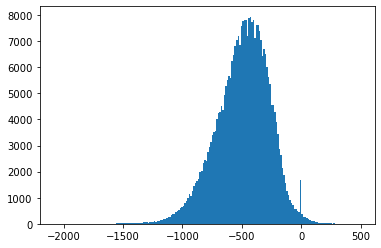
\includegraphics[width=0.3\linewidth]{images/rec_100_hist_measurements_200_bins.png}}
    \hfill
  \subfloat[Record 102]{%
  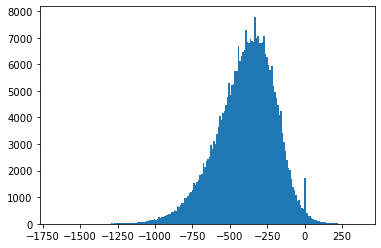
\includegraphics[width=0.3\linewidth]{images/rec_102_hist_measurements_200_bins.png}}
    \hfill
  \subfloat[Record 115]{%
  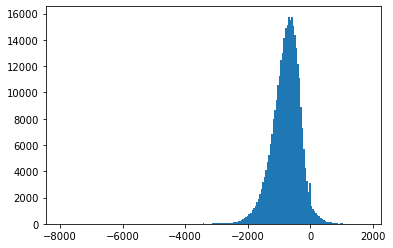
\includegraphics[width=0.3\linewidth]{images/rec_115_hist_measurements_200_bins.png}}
    \\
  \subfloat[Record 202]{%
  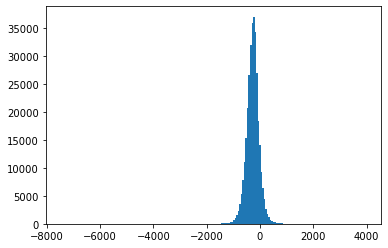
\includegraphics[width=0.3\linewidth]{images/rec_202_hist_measurements_200_bins.png}}
    \hfill
  \subfloat[Record 208]{%
  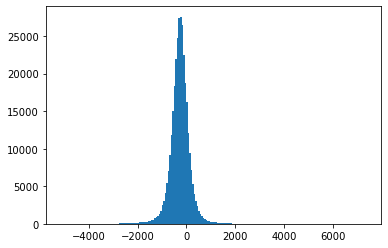
\includegraphics[width=0.3\linewidth]{images/rec_208_hist_measurements_200_bins.png}}
    \hfill
  \subfloat[Record 234]{%
  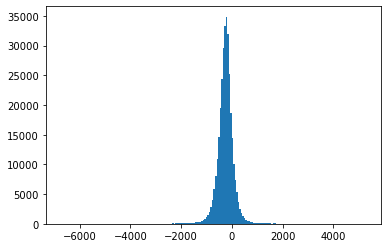
\includegraphics[width=0.3\linewidth]{images/rec_234_hist_measurements_200_bins.png}}
  \caption{Histograms of measurement values with the sparse binary sensing matrix
  with $m=256,n=512,d=4$ in 200 bins}
\label{fig:cs:codec:y:hist:200}
\end{figure*}


\begin{figure}[htb]
    \centering % <-- added
  \centering 
  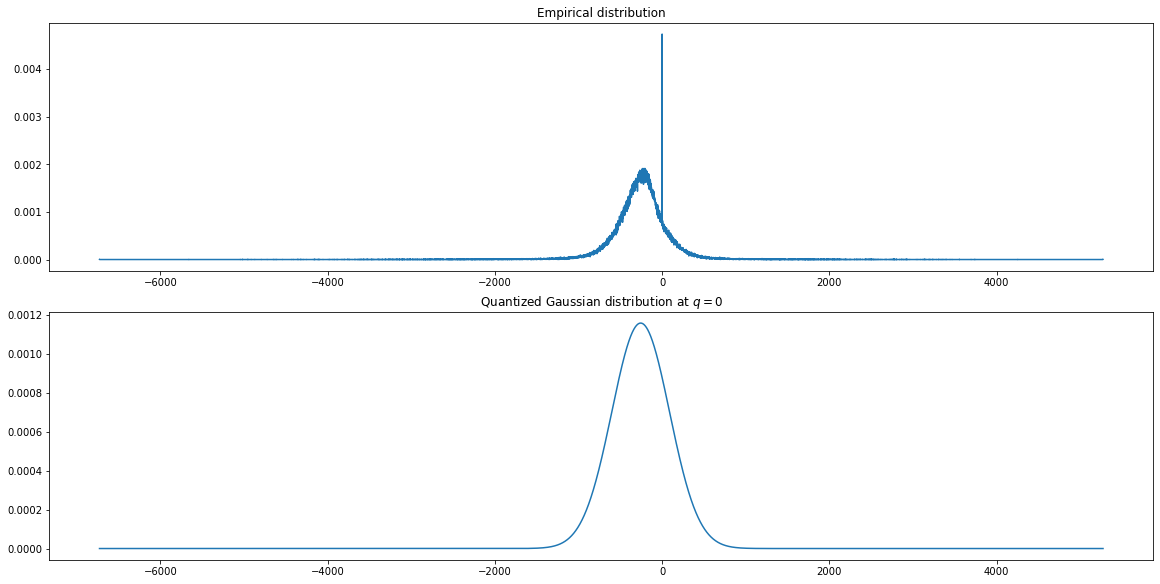
\includegraphics[width=0.95\linewidth]
  {images/rec_234_empirical_vs_quantized_gaussian.png}
\caption{Empirical and quantized Gaussian distributions for measurement values
$\by$ in record 234}
\label{fig:cs:codec:y:234:empirical:quantized}
\end{figure}

\subsubsection{Clipping}

An entropy coder can handle with a finite set of symbols
only. Hence, the range of input values [measurements
coded as integers] must be restricted to a finite range.
This is the reason one has to choose a distribution
with finite support (like quantized Gaussian).
From \cref{tbl:cs:codec:measure:stats} one can see that
while the complete range of measurement values can be
up to 40-50x larger than the standard deviation, the iqr
is less than $1.5$ times the standard deviation. In other
words, the measurement values are fairly concentrated
around its mean. This can be visually seen from the
histograms in \Cref{fig:cs:codec:y:hist:200} also.

\subsubsection{Quantization}

\Cref{fig:100:q:0-7} demonstrates the impact of the
quantization step on the reconstruction quality
for record 100 under non-adaptive quantization.
$6$ windows of $512$ samples
were used in this example. The first panel
shows the original (digital) signal. Remaining
panels show the reconstruction at different
quantization parameters.
The reconstruction visual quality is excellent
up to $q=5$ (PRD below 7\%), good at $q=6$ (PRD at 9\%)
and clinically unacceptable at $q=7$
(with PRD more than 15\%).
One can see significant waveform distortions at $q=7$.
Also note how the quality score keeps increasing till
$q=4$ and starts decreasing after that with a massive
drop at $q=7$.



\begin{figure}[!ht]
\centering 
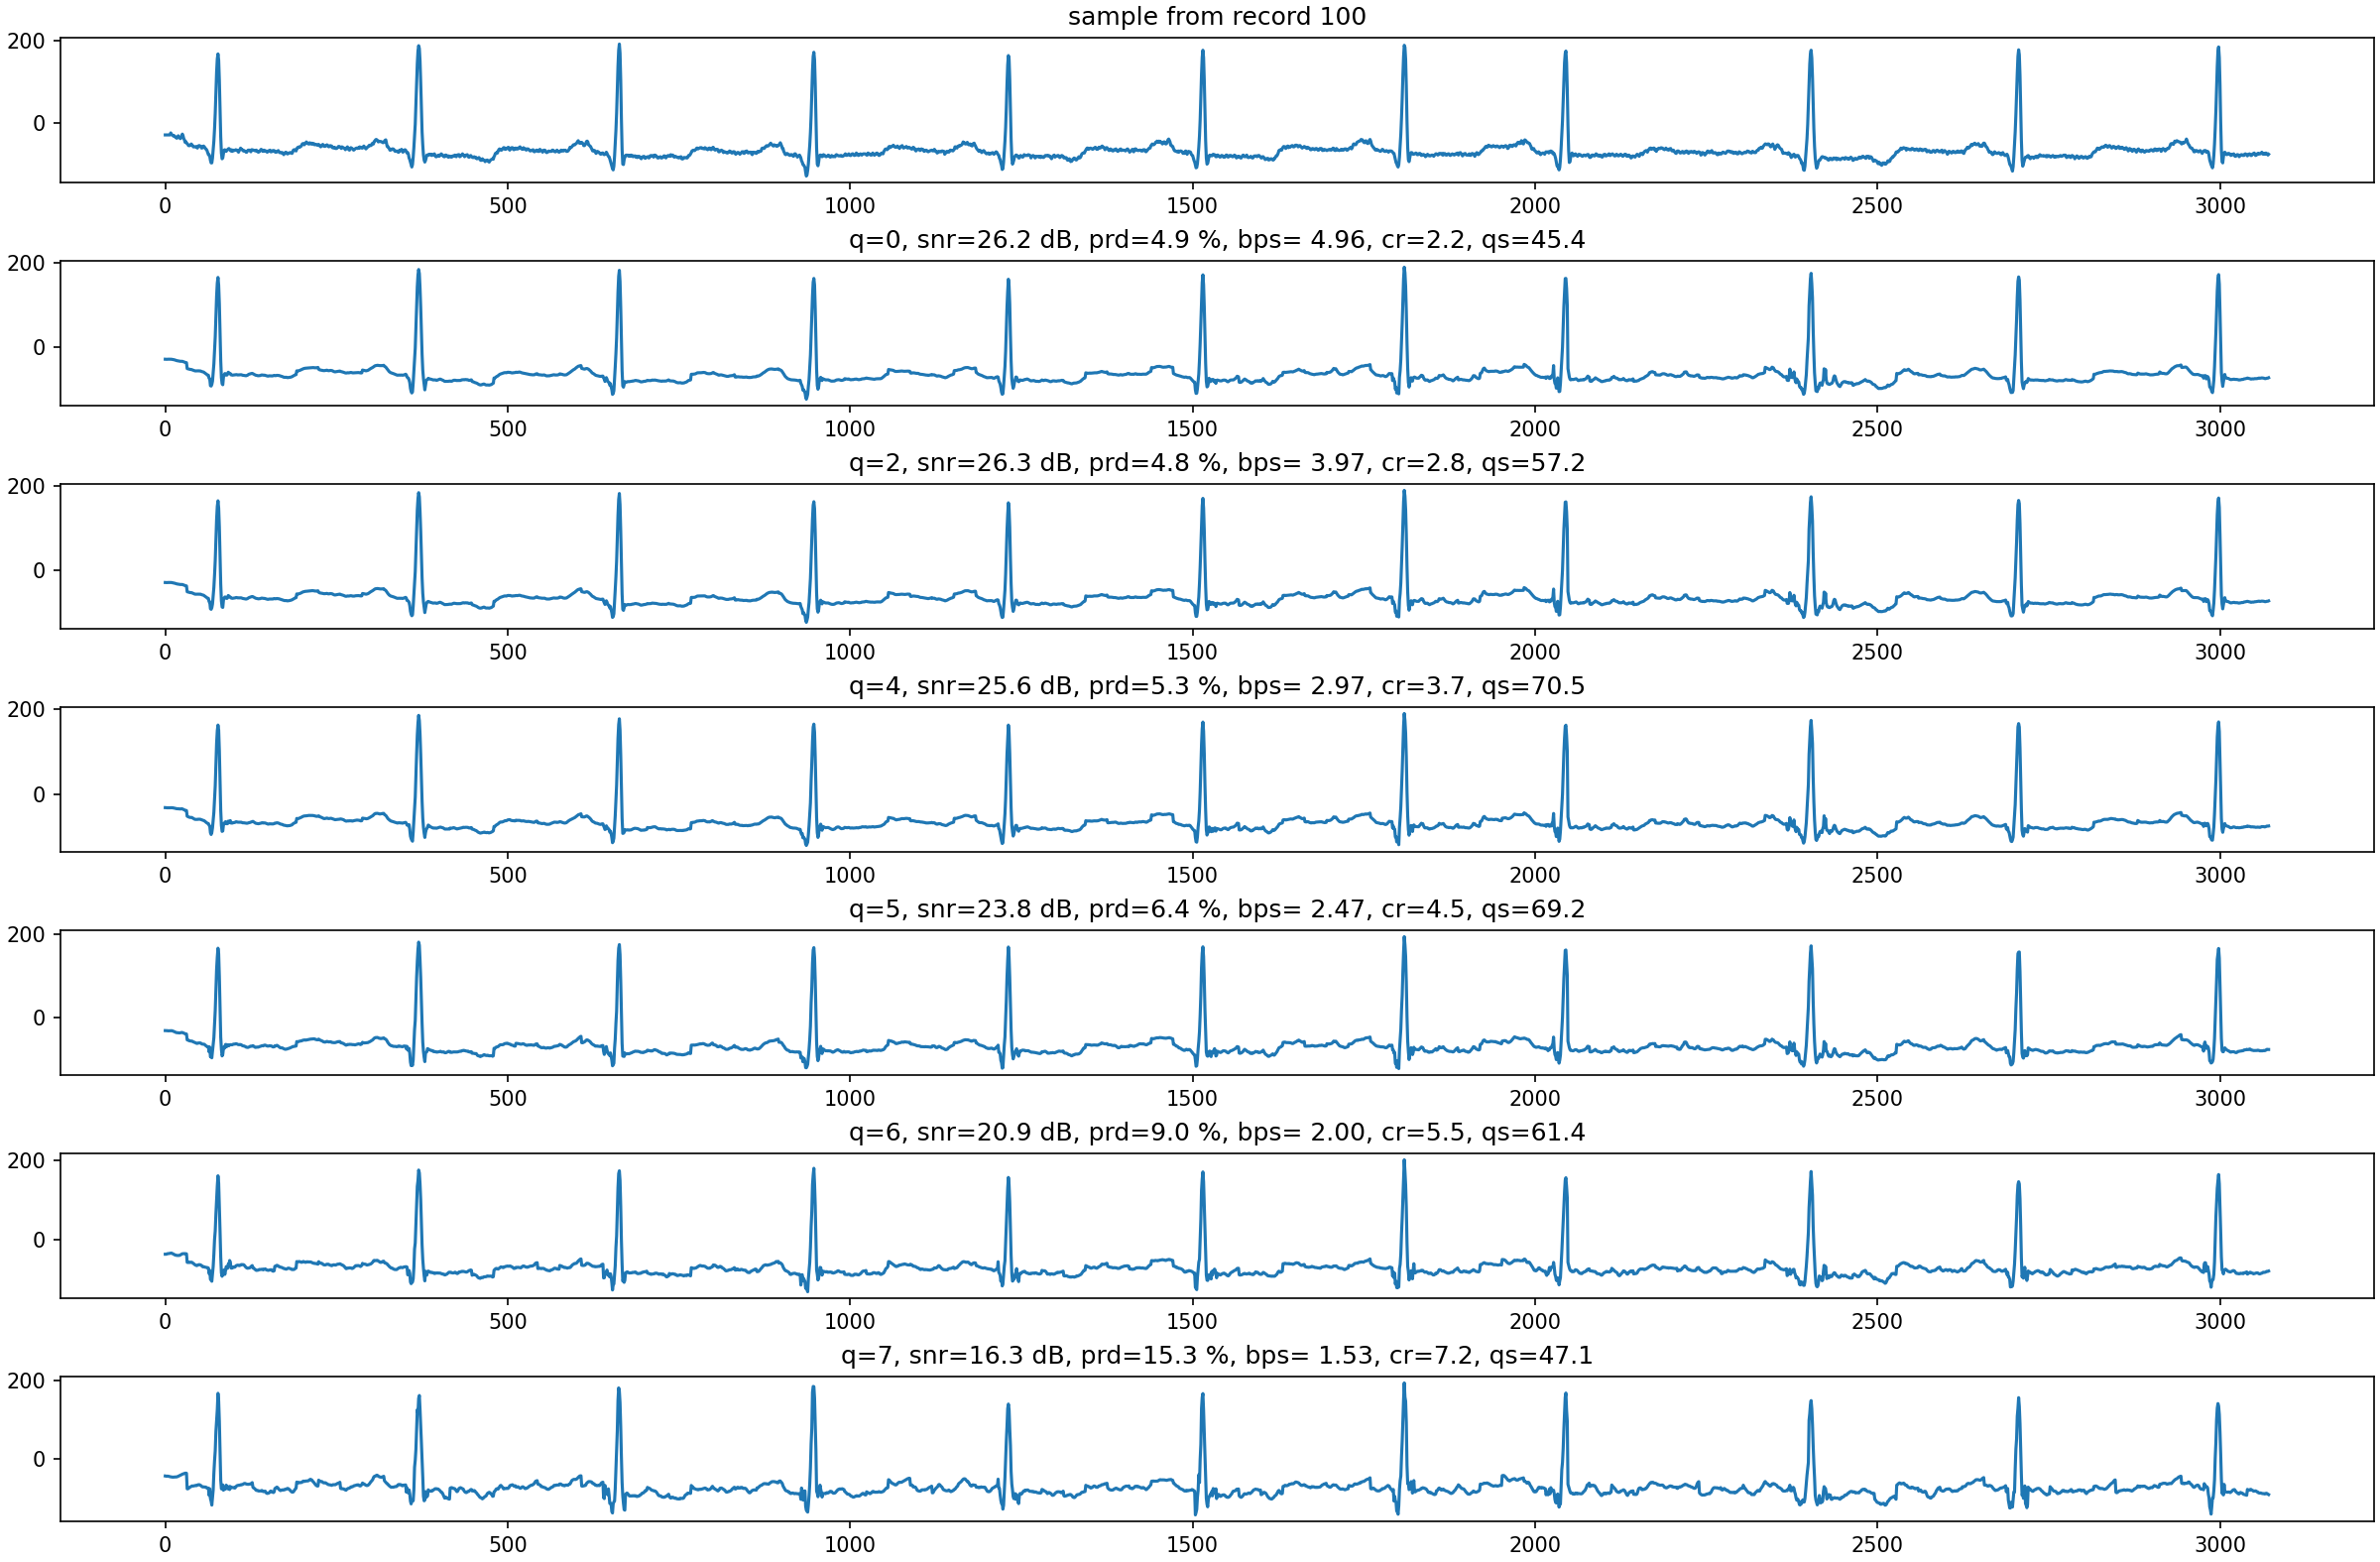
\includegraphics[width=0.95\linewidth]
{images/rec_100_q_cr_prd_qs.png}
\caption{Reconstruction of a small segment of record 100
for different values of $q=0,2,4,5,6,7$ with $m=256,n=512,d=4$
under non-adaptive quantization.
Block size for the BSBL-BO decoder is $32$.}
\label{fig:100:q:0-7}
\end{figure}
